\chapter{Modello di Markowitz}
\section{Introduzione}
Questa introduzione è necessaria per spiegare il contesto in cui ci troviamo. Stiamo introducendo la Teoria di Markowitz, una teoria matematica per la costruzione di portafogli di titoli ottimizzati. Sono necessarie però un po’ di definizioni, a partire da quella di portafoglio di titoli.
Un portafoglio di titoli è un insieme di titoli finanziari, ovvero un insieme di azioni acquistabili nei vari possibili mercati finanziari. A ogni titolo presente nel portafoglio è associato un peso che è la percentuale di capitale a disposizione investito sul titolo, sul totale di capitale investito su tutti i titoli presenti nel portafoglio, quindi quanto ho investito su un cero titolo rispetto agli altri titoli presenti nel portafoglio.\\
Per ogni titolo sono importanti da considerare due parametri: il rischio e il rendimento.\\
Il rischio è legato alla varianza, la volatilità dei prezzi, ovvero quanto i valori storici si discostano dalla media, più un titolo è stabile (cresce e diminuisce poco) più è sicuro, più un titolo ha massimi e minimi distanti ( e quindi cresce e diminuisce tanto) più è incerto e ha rischio alto.\\
Il rendimento di un titolo è quanto il titolo ti può far guadagnare, più è alto il rendimento di un titolo, più si guadagna vendendolo. Il rendimento che generalmente si utilizza è detto lineare ed è il rendimento percentuale, ovvero il rendimento attuale in funzione del prezzo precedente e si calcola con la formula:\\
\formula{Rendimento percentuale}{
\[ rendimento = \frac{prezzo~attuale - prezzo~precedente}{prezzo~precedente}   \]
}
\noindent
Questa formula descrive proprio il concetto di rendimento, facendo un esempio pratico il "prezzo~precedente" potrebbe rappresentare il prezzo di acquisto, mentre il "prezzo~attuale" potrebbe rappresentare il prezzo di vendita, applicando la formula scopro in percentuale quanto ho guadagnato dall'operazione, ovvero il mio rendimento.\\
Markowitz considera al posto del rendimento, il rendimento atteso, cioè quanto l’investitore si aspetta di ottenere da uno o più titoli nel futuro. Ovviamente, poiché si tratta di un valore atteso, il rendimento realizzato potrebbe differire dal reale in quanto viene misurato riferendosi allo storico del titolo. Un criterio semplice potrebbe essere considerare il rendimento atteso pari al rendimento medio che il titolo ha registrato in passato. \\
Il rendimento medio è ottenuto tramite lo “stimatore della media”, che nel nostro caso è semplicemente la media aritmetica. La formula quindi è:\\
\formula{Rendimento medio}{\[ rendimento = \frac{prezzo_1 + prezzo_2 + ... + prezzo_n}{n} \]}
\noindent
Una raffinazione successiva potrebbe essere limitare l’analisi passata a un periodo minore di tutto lo storico e finanziariamente simile al periodo futuro in cui si vuole investire (ad esempio momenti di crisi o momenti di crescita). \\

\begin{Nota}
 Nota: Nella maggior parte dei casi non si potrà mai avere una stima della media affidabile, poiché per avere un valore affidabile servirebbero circa 90 anni di dati. Si può quindi scegliere di selezionare un periodo lungo probabilmente complessivamente poco simile al periodo di investimento o un periodo più corto e simile al periodo di investimento, ma con meno dati e quindi meno preciso.\\
\end{Nota}
\noindent
Tornando alla teoria di Markowitz, con portafoglio di ottimo si intende quella serie di pesi (ognuno legato a un titolo presente nel portafoglio) per cui complessivamente il portafoglio avrà il massimo rendimento atteso e il minimo rischio, ovvero la minima varianza.\\
Abbiamo quindi ora i concetti base per spiegare la teoria di Markowitz.

\vspace{1cm}
\section{Teoria del modello di Markowitz}

La teoria di Markowitz prende il nome dal suo ideatore, Henry Markowitz (Chicago, 24 agosto 1927)  economista statunitense che vinse nel 1990 il premio Nobel per l’economia. 
Markowitz sosteneva che per costruire un portafoglio occorre individuare titoli la cui combinazione minimizzi il rischio e massimizzi il rendimento; per fare ciò fu il primo a introdurre il concetto di correlazione fra i titoli.
Oltre al rischio del singolo titolo, è importante considerare il rischio di un portafoglio composto da due o più titoli, il quale dipende dalla correlazione esistente tra essi. Se non esiste alcuna correlazione tra i diversi titoli, il rischio di portafoglio sarebbe analogo a quello dei singoli titoli, questo perché non vi è covarianza, come si vede dalla formula del rischio del portafoglio.

\formula{Covarianza}{\[ covarianza = \sum{\frac{(x_i - media(x)) \ast (y_i - media(y))}{n-1}} \]}
\begin{Nota}
 Nota: n $\rightarrow$ numero dei dati\\
\end{Nota}

\noindent
Considerando due titoli e il loro coefficiente di correlazione, se questo è positivo o negativo la crescita del rendimento di un titolo corrisponde l’aumento o decremento del rendimento del secondo titolo. Si deduce che nel caso di andamenti contrapposti dei rendimenti dei titoli – ovvero il concetto di diversificazione – il rischio globale di un portafoglio si riduce perché si va a ridurre il rischio “idiosincatico” a zero (ovvero il rischio legato all’andamento del singolo titolo, annullabile diversificando), rimane intatto però il rischio “di mercato” (ovvero il rischio sistematico che non può essere ridotto poiché dato dall’incertezzza del mercato data da eventi esterni ), che non può essere eliminato in nessun caso poiché intrinseco al mercato stesso. In parole povere se riesco a inserire titoli ben correlati tra di loro il rischio globale diminuisce poiché se un titolo scende, e quindi perde valore, i titoli a lui correlati salgono, e quindi acquistano valore, compensandosi.
Il modello di Markowitz serve a tracciare una curva che descrive tutte le possibili combinazioni di titoli all’interno del portafoglio. Questa curva è chiamata “frontiera efficiente”  poiché mostra quale è la volatilità minima associata a ogni livello di  rendimento atteso.\\
Ogni punto della curva è un possibile combinazione del portafoglio e andando a vedere le coordinate di ogni punto abbiamo sulla x la varianza e sulla y il rendimento.

\begin{figure}[!ht]
    \centering
    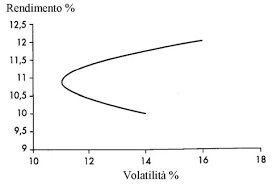
\includegraphics[scale=1.2]{pictures/grafico_markowitz.png}
    \caption{Curva di Markowitz}
    \label{Curva di Markowitz}
\end{figure}

\noindent
In questa curva abbiamo 3 parti di interesse:
\begin{enumerate}
\item[-] La prima è la parte di curva che tende verso il basso e verso destra, questa parte è da ignorare, poiché, come si vede dal grafico il rendimento di un portafoglio diminuisce all’aumentare della volatilità, nessun investitore investirebbe in un tale portafoglio (e quindi in una tale combinazione di titoli. Inoltre guardando il grafico si nota che a parità di volatilità c’è un maggiore valore di rendimento, ciò ci porta alla seconda parte interessante.
\item[-] La seconda parte della curva di interesse è la parte che tende verso l’alto e verso destra, è detta “frontiera efficiente” poiché descrive solo i portafogli il cui investimento può essere interessante per un investitore che desidera massimizzare il rendimento, anche a costo di aumentare la volatilità. Questa parte comprende quindi solo i portafogli che per ogni livello di volatilità offrono il rendimento più elevato possibile.
\item[-] La terza è un punto, è la combinazione che compone il “portafoglio a varianza minima globale” (o “portafoglio a volatilità minima globale”), graficamente è il punto più a sinistra nella curva e descrive il portafoglio con il rischio minimo.
\end{enumerate}


\noindent
Note matematiche:
\begin{enumerate}
    \item[-] A noi interessa la curva, ma in realtà i punti che compongono l’area interna alla curva sono anch’essi delle combinazioni di titoli del portafogli, ma non sono quelle efficienti a parità di volatilità. L’area interna è chiamata “opportunity set”.
    \item[-] Nella realtà la curva è considerata finita, ma nella teoria matematica si può espandere verso l’alto all’infinito. Chiaramente questo implica che il rendimento e il rischio. assumeranno valori molto alti. Per eguagliare un rendimento molto altro l’investitore potrà vendere allo scoperto, assumendo una posizione di short contro il titolo, a questo però corrisponderà un rischio >1, ciò significa che se perde, perderà più capitale di quello che ha investito.
\end{enumerate}

\noindent
Da questa teoria matematica si parte per risolvere il problema dell’ottimizzazione, poiché fissato un certo rendimento desiderato basterà prendere sulla curva il punto corrispondente a quel rendimento (si ricorda che a ogni punto corrisponde una combinazione di pesi, prendere un punto vuol quindi dire utilizzare quei pesi).

\vspace{1cm}
\section{Metodo “a mano”}

Per utilizzare la teoria di Markowitz si parte da un vettore contenete i rendimenti medi per ogni titolo che si vuole inserire nel portafoglio e una matrice di covarianze, in cui ogni posizione [i,j] conterrà la covarianza tra il titolo i e il titolo j, si noti che la diagonale contiene le varianze dei singoli titoli, essendo che covarianza(titolo i, titolo i) == varianza(titolo i). Nell’utilizzo al computer questi dati ce li calcoliamo, negli esercizi svolti a mano generalmente questi due dati (vettore medie e matrice covarianze) vengono dati dal problema.\\
Imposto poi il sistema. Si tratta di un sistema di ottimo vincolato con una funzione obbiettivo convessa, che è la lagrangiana:

\formula{Lagnangiada~di~Markowitz}{
\[ L(\lambda_1, \lambda_2,x) = x^TVx + \lambda_1 (m - \mu^Tx) + \lambda_2 (1- e^Tx) \]
}
\noindent
Risolvendo il sistema riesco cosi a ottenere la curva (che è una iperbole) in funzione di a, b e c descritta dalla seguente formula:
\formula{Curva~di~Markowitz}{\[\sigma = \sqrt{\frac{cm^2-2bm+a}{ac-b^2}}\]}

Con a, b, c:
\noindent
\formula{Parametro a}{\[ a = \mu^T * V^{-1} * \mu\]}
\formula{Parametro b}{\[b = \mu^T * V^{-1} * e \]}
\formula{Parametro c}{\[c = e^T * V^{-1} * e \]}



\begin{Nota}
    Didascalia:
    \begin{enumerate}
        \item[-] V $\rightarrow$ matrice delle covarianze
        \item[-] $\mu \rightarrow$ vettore delle medie dei titoli
        \item[-] e $\rightarrow$ vettore sommatoria\\
    \end{enumerate}

    Reminder delle operazioni:
    \begin{enumerate}
        \item[-] $x^T \rightarrow$ x trasposto
        \item[-] $x^{-1} \rightarrow$ x inverso
    \end{enumerate}
\end{Nota}



\noindent
Questa formula descrive la curva del rischio in funzione di m, ovvero il rendimento atteso.\\
Da questa formula parto per riscrivere una seconda formula per trovare la x,ovvero il vettore dei pesi, in funzione di m, ovvero il rendimento atteso.


\formula{Vettore~dei~pesi}{\[ x = \frac{((m*c-b) * \mu^T * V^{-1} * (a-m*b)*e^T*V^{-1})^T}{ a*c-b^2 }\]}



\noindent
Impostando quindi in questa formula una certa m a scelta e i valori di a,b e c calcolati con le formule precedentemente presentate è possibile trovare sulla curva il punto che possiede il rendimento corrispondente e un certo vettore dei pesi che a noi interessa.\\
Si noti che vi è un certo rendimento minimo, infatti prendendo solo il ramo dell’iperbole maggiore del punto detto “portafoglio a varianza minima globale” non sarà possibile ottenere un rendimento minore del rendimento associato a questo punto. Bisogna così calcolarsi m*, ovvero il rendimento del “portafoglio a varianza minima globale”, e verificare che il rendimento atteso sia maggiore di m*  

\vspace{1cm}
\section{Dalla penna al computer}
\subsection{processo di sviluppo dello pseudocodice}
Visto come si esegue questo calcolo a mano si tenta di tradurre questa serie di passaggi in algoritmo.
Innanzitutto a noi interessa x, ovvero il vettore dei pesi, calcolato con\\
\[ x = \frac{((m*c-b) * \mu^T * V^{-1} * (a-m*b)*e^T*V^{-1})^T}{ a*c-b^2 }   
\]\\
\noindent
per risolvere questa formula abbiamo bisogno di m, a, b, c, $\mu$ (array medie titoli), V (matrice covarianza) e e(vettore sommatoria).\\
M viene richiesta come input quindi ce l’abbiamo. Abbiamo bisogno di a,b,c che, dalle formule scritte sopra, per essere calcolati hanno bisogno di mu e V come input.\\
V e $\mu$ non ce li abbiamo e per ricavarli utilizziamo i dati grezzi. Partiamo quindi da calcolare $\mu$ e V a partire dai valori di chiusura medi settimanali. \\
I valori di chiusura medi settimanali si recuperano da delle API che prendono i dati da dei database (ad esempio tramite una api di yahoo finance). Sono la media dei prezzi di una azione al momento della chiusura del mercato, prendendo il prezzo in ogni giorno nell’arco di una settimana e facendone la media si ottiene il valore di chiusura medio di una settimana per una certa azione.\\ 
Noi quindi per calcolare i dati necessari impostiamo un certo periodo di tempo in cui verrà fatta l’analisi e andiamo a recuperare per i titoli selezionati i valori di chiusura media di ogni settimana. Si ricorda che il periodo passato analizzato dovrebbe essere simile al periodo futuro in cui verrà fatto l’investimento.\\

\noindent
Ottenuta questa grande matrice contenente i titoli e i relativi prezzi di chiusura settimanali andiamo a calcolare $\mu$ e V.\\ 
Per calcolare $\mu$ facciamo la media aritmetica dei prezzi per ogni titolo, otteniamo così un’array lungo quanto la quantità di titoli contenente in ogni posizione la media di un certo tiolo. \\
Per calcolare V si utilizza la varianza e la covarianza. La posizione \code{V[i,j]} è infatti data dalla covarianza tra \code{titolo[i]} e \code{titolo[j]} presenti nella matrice delle chiusure settimanali, quindi la funzione \code{covarianza()} prende in input due array, che devono essere della stessa dimensione, contenenti i prezzi di chiusura settimanali e ne calcola un numero, che è la covarianza. Da notare che la covarianza tra \code{titolo[i]} e \code{titolo[i]} (quindi la covarianza tra lo stesso titolo) è uguale alla varianza di quel titolo. Otteniamo quindi una matrice che ha sulla diagonale (dove i==j) ha le varianze dei singoli titoli e nelle altre posizioni tutte le covarianze, da notare che è una matrice che si può specchiare sulla diagonale poiché la covarianza tra i e j è uguale alla covarianza tra j e i.\\

\noindent
Adesso possiamo calcolare a, b e c con le formule:

\noindent
\[a = \mu^T * V^{-1} * \mu\] 
\[b = \mu^T * V^{-1} * e \]
\[c = e^T * V^{-1} * e \]

\noindent
Può essere necessario alla comprensione spiegare cosa sono il vettore sommatoria e una lista trasposta. Una generica matrice trasposta è una matrice in cui le righe vengono sostituite dalle colonne e viceversa, quindi l’effetto di trasposizione su una lista colonna (ovvero un array) mi farà ottenere una matrice con tante colonne quante righe del vettore e ogni colonna conterrà un solo elemento. \\
Il vettore sommatoria è un vettore composto da solo 1, è detto sommatoria poiché se moltiplicato (o meglio post-moltiplicato) per un altro vettore il risultato che si ottiene è la sommatoria del primo vettore, si ricorda che la moltiplicazione tra vettori, il primo verticale e l’altro orizzontale, è data dalla sommatoria delle moltiplicazioni tra i valori nella stessa posizione dei due vettori.\\

\noindent
Ora che abbiamo $\mu$, V, a,b, e c calcoliamo m* per verificare che l’m richiesto sia maggiore, e quindi il calcolo sia effettuabile.\\
Con questa formula possiamo calcolare m*:
\formula{Parametro m*}{\[ m* = \frac{-B}{2*C} \]}
con:
\formula{Parametro B}{\[ B = \frac{2*b}{a*c-b^2}\]}
\formula{Parametro C}{\[C = \frac{c}{a*c-b^2}\]}
\noindent
Se m>m* allora si può procedere a calcolare la x con la formula già data in precedenza
\[ x = \frac{((m*c-b) * \mu^T * V^{-1} * (a-m*b)*e^T*V^{-1})^T}{ a*c-b^2 }\]
\\
\noindent
Si ottiene così un vettore contenente i pesi di ogni titolo. Da notare che questo vettore rappresenta la percentuale di capitale da investire in ogni titolo, la sommatoria del vettore quindi deve essere teoricamente 1, in realtà però sarà circa 1 (può non essere esattamente uno a causa dell’approssimazione). Se il peso relativo al titolo è positivo bisognerà acquistare quel titolo utilizzando una percentuale del capitale da investire corrispondente al peso, se il peso è negativo bisognerà vendere allo scoperto quel titolo in quantità pari alla percentuale del capitale corrispondente al peso.

\newpage
\subsection{Pseudocodice}


\begin{minted}{java}


//lista contenente i nomi dei titoli che 
//si desidera inserire nel portafoglio
title_list = [ "title1", "title2", "title3" ] 

//dati grezzi dei titoli
raw_title_matrix = get_rew_datas(title_list)

//si calcola l'array delle medie
a_mean = [] //array delle medie
foreach( title in raw_prices_matrix ){
	a_mean[title] = mean(raw_prices_matrix [title])
}

//calcolo la matrice di covarianza
matrix_covar = [] //matrice covarianza
for( i in length(title_list)){
	row = [] //lista in cui si accumulano i risultati
	for (j in length(title_list)){
		if (i==j){
			row.append( varianza(raw_title_matrix[i] )
		}else{
			row.append(covarianza(raw_title_matrix[i],
			                        raw_title_matrix[j] )
		}	
	}
	matrix_covar.append(row)
}

//calcolo i parametri utili
a = find_a(a_mean, matrix_covar)
b = find_b(a_mean, matrix_covar)
c = find_c(matrix_covar)
B = find_B(a,b,c)
C = find_C(a,b,c)

//calcolo m*
m* = find_m*(B,C)

//verifico se m richiesto è valido
if(m*>m){
	return null //impossibile calcolare il risultato
}

//qua m è accettabile per il calcolo
 
\end{minted}
 \begin{Nota}
 A questo punto applico la formula: $x = \frac{((m*c-b) * \mu^T * V^{-1} * (a-m*b)*e^T*V^{-1})^T}{ a*c-b^2 }$
 \end{Nota}
\begin{minted}{java}

parz_1= mul_array_matrix( mul_scalar_vector((m*c-b), traspose(mu)),
                                inverse(V))
parz_2= mul_array_matrix( mul_scalar_vector((a-m*b), traspose(vect_sum)),
                                inverse(V))  
num = sum_vectors( traspose(parz_1), parz_2)
num_traspose = traspose(num) 
denom = (a*c)-(b*b) 

x = div_array_scalar( num_traspose, denom )
// a questo punto x è una lista contenente tutti i pesi

//da qua si fanno delle operazioni di controllo e formattazione

//controllo che la sommatoria dell’array sia =1
if(summation(x) not 1){
    return null
}else{
//ritorno l'array contenente i pesi
    return x
}
    
\end{minted}

